
\documentclass[12pt, svgnames, titlepage]{report}

\title{Learning Python and Embedded Software 1 Packet Demo}
\textwidth=7in
\textheight=9.5in
\topmargin=-1in
\headheight=0in
\headsep=.5in
\hoffset  -.85in


\usepackage{hyperref}
\hypersetup{
    colorlinks,
    citecolor=black,
    filecolor=black,
    linkcolor=black,
    urlcolor=black
}

%\usepackage[T1]{fontenc}
%\usepackage{txfonts}
\usepackage{fancyhdr}
\usepackage{enumitem}
\pagestyle{fancyplain}
\usepackage{xcolor}
\definecolor{UCLABlue}{RGB}{83, 104, 149}
\definecolor{UCLAGold}{RGB}{254, 187, 54}

\author{Philip Tracton} 
%\date{\today}
\date{}

\usepackage{tikz}
\usepackage{pgf}
\usetikzlibrary{arrows,automata}
\usepackage[latin1]{inputenc}
\usepackage{verbatim}
\usepackage{kpfonts}
\usepackage[explicit]{titlesec}
\newcommand*\chapterlabel{}
\titleformat{\chapter}
  {\gdef\chapterlabel{}
   \normalfont\sffamily\Huge\bfseries\scshape}
  {\gdef\chapterlabel{\thechapter\ }}{0pt}
  {\begin{tikzpicture}[remember picture,overlay]
    \node[yshift=-3cm] at (current page.north west)
      {\begin{tikzpicture}[remember picture, overlay]
        \draw[fill=UCLABlue] (0,0) rectangle
          (\paperwidth,3cm);
        \node[anchor=east,xshift=.9\paperwidth,rectangle,
              rounded corners=20pt,inner sep=11pt,
              fill=UCLAGold]
              {\color{white}\chapterlabel#1};
       \end{tikzpicture}
      };
   \end{tikzpicture}
  }
\titlespacing*{\chapter}{0pt}{50pt}{-60pt}

\lfoot{\colorbox{UCLABlue}{\textcolor{white}{P. Tracton}}}
\cfoot{\colorbox{UCLABlue}{\textcolor{white}{Packet Demo}}}
\rfoot{\colorbox{UCLABlue}{\textcolor{white}{\thepage}}}


\usepackage{array}
\newcolumntype{L}[1]{>{\raggedright\let\newline\\\arraybackslash\hspace{0pt}}m{#1}}

\usepackage{graphicx}
\usepackage[export]{adjustbox}

% Margins
\topmargin=-0.45in
\evensidemargin=0in
\oddsidemargin=0in
\textwidth=6.5in
\textheight=9.0in
\headsep=0.25in

\linespread{1.1} % Line spacing

% Set up the header and footer
%\pagestyle{fancy}
%\lfoot{Embedded Software 1} % Bottom left footer
%\cfoot{} % Bottom center footer
%\rfoot{Page\ \thepage\ of\ \protect\pageref{LastPage}} % Bottom right footer
\renewcommand\headrulewidth{0.4pt} % Size of the header rule
\renewcommand\footrulewidth{0.4pt} % Size of the footer rule

\setlength\parindent{0pt} % Removes all indentation from paragraphs

%----------------------------------------------------------------------------------------
%	NAME AND CLASS SECTION
%----------------------------------------------------------------------------------------

\newcommand{\hmwkTitle}{Packet Demo} % Assignment title
\newcommand{\hmwkClass}{Learning Python and \\Embedded Software 1} % Course/class
%\newcommand{\hmwkClassTime}{Online} % Class/lecture time
\newcommand{\hmwkClassInstructor}{Philip Tracton} % Teacher/lecturer
\newcommand{\hmwkAuthorName}{} % Your name

%----------------------------------------------------------------------------------------
%	TITLE PAGE
%----------------------------------------------------------------------------------------

\title{
\vspace{2in}
\textmd{\textbf{\hmwkClass\ \\ \hmwkTitle}}\\
\vspace{0.1in}\normalsize{Instructor: \textit{\hmwkClassInstructor}}\\
%\normalsize\vspace{0.1in}\textcolor{red}{\large{Due\ on\ \hmwkDueDate}}\\
%\vspace{3in}
}
\author{\textbf{\hmwkAuthorName}}
\date{} % Insert date here if you want it to appear below your name

%----------------------------------------------------------------------------------------



\begin{document}

\maketitle


\tableofcontents
\newpage

\chapter{Introduction and GOALS}
\section{Introduction}
\noindent Both Learning Python and Embeded Software 1 have a lot of material to cover.  I can not go over everything nor do I present whole applications to either class.  We go over blocks of code and make some small programs.  This is a demonstration of the beginning of a pair of applications.  There is 1 application that is written in Python 3 and runs on your PC.  There is a second application that is written in C and runs on your \underline{\href{http://www.st.com/web/en/catalog/tools/FM116/SC959/SS1532/PF254044}{STM32F3 Discovery board}}.  \\

\vspace{0.5cm}
\noindent Unless you have taken both classes with me, it is unlikely that you have all of the equipment to run these applications together.  That's ok, this is meant to show you coding in both langauges that was a bit too large for either course.  \\

\chapter{Embedded Software}
\section{Resources}
This example requires the following components:
\begin{enumerate}
\item The \underline{\href{http://www.st.com/web/en/catalog/tools/FM116/SC959/SS1532/PF254044}{STM32F3 Discovery board}}
\item \underline{\href{http://www.monoprice.com/Product?c_id=103&cp_id=10303&cs_id=1030302&p_id=8635&seq=1&format=2}{USB A to Mini-B cable}}
\item \underline{\href{http://www.amazon.com/gp/product/B00CD264HG/ref=oh_aui_detailpage_o04_s00?ie=UTF8&psc=1}{USB A to RS232 cable and board}} and \underline{\href{http://www.silabs.com/products/interface/usbtouart/Pages/usb-to-uart-bridge.aspx}{device drivers for it}}.
\item \underline{\href{http://www.keil.com/download/product/}{KEIL IDE}}.  This tool only runs on Windows, it does not run on Mac OS or Linux.
\item The \underline{\href{https://github.com/ptracton/packet_demo}{code}} from my Git repository.  It has this document, embedded software and python code.
\end{enumerate}
\newpage


\section{Code}

\noindent The design from the class was a CLI.  This was pretty simply on the target and on the PC side.  On the PC, putty or another terminal emulator, could be used to send strings of commands to the target.  This is hard to use since you had to type in a lot of commands and our CLI was not forgiving of typos.  It was also easy to slip in bad commands since whatever you typed went to the target and required the target to sanitize the inputs.  This puts extra burden on the target.\\

\vspace{0.5cm}

\noindent A different approach is what we are taking in this demonstration.  The CLI code is removed.  It is replaced with the Packet Handling code.  Putty or another terminal emulator is not needed.  They have been replaced with a python script that gives the user a GUI interface.  Instead of typing commands, the user can click on buttons.  This is an easier interface for users.  It allows for input sanitization to be done on the PC, removing this load from the target.  The challenge to this approach is that a new application for the PC now must be written and maintained and rolled out to the PCs that host the targets.  The 2 most common tools I see for this are LabView and Python.  Since I teach both the embedded software and python courses I thought I would put together a demonstration of Python controlling an embedded target.  \\

\vspace{0.5cm}
\noindent The code on the target is very similar to that used in the course.  

\subsection{Packet RX State Machine}


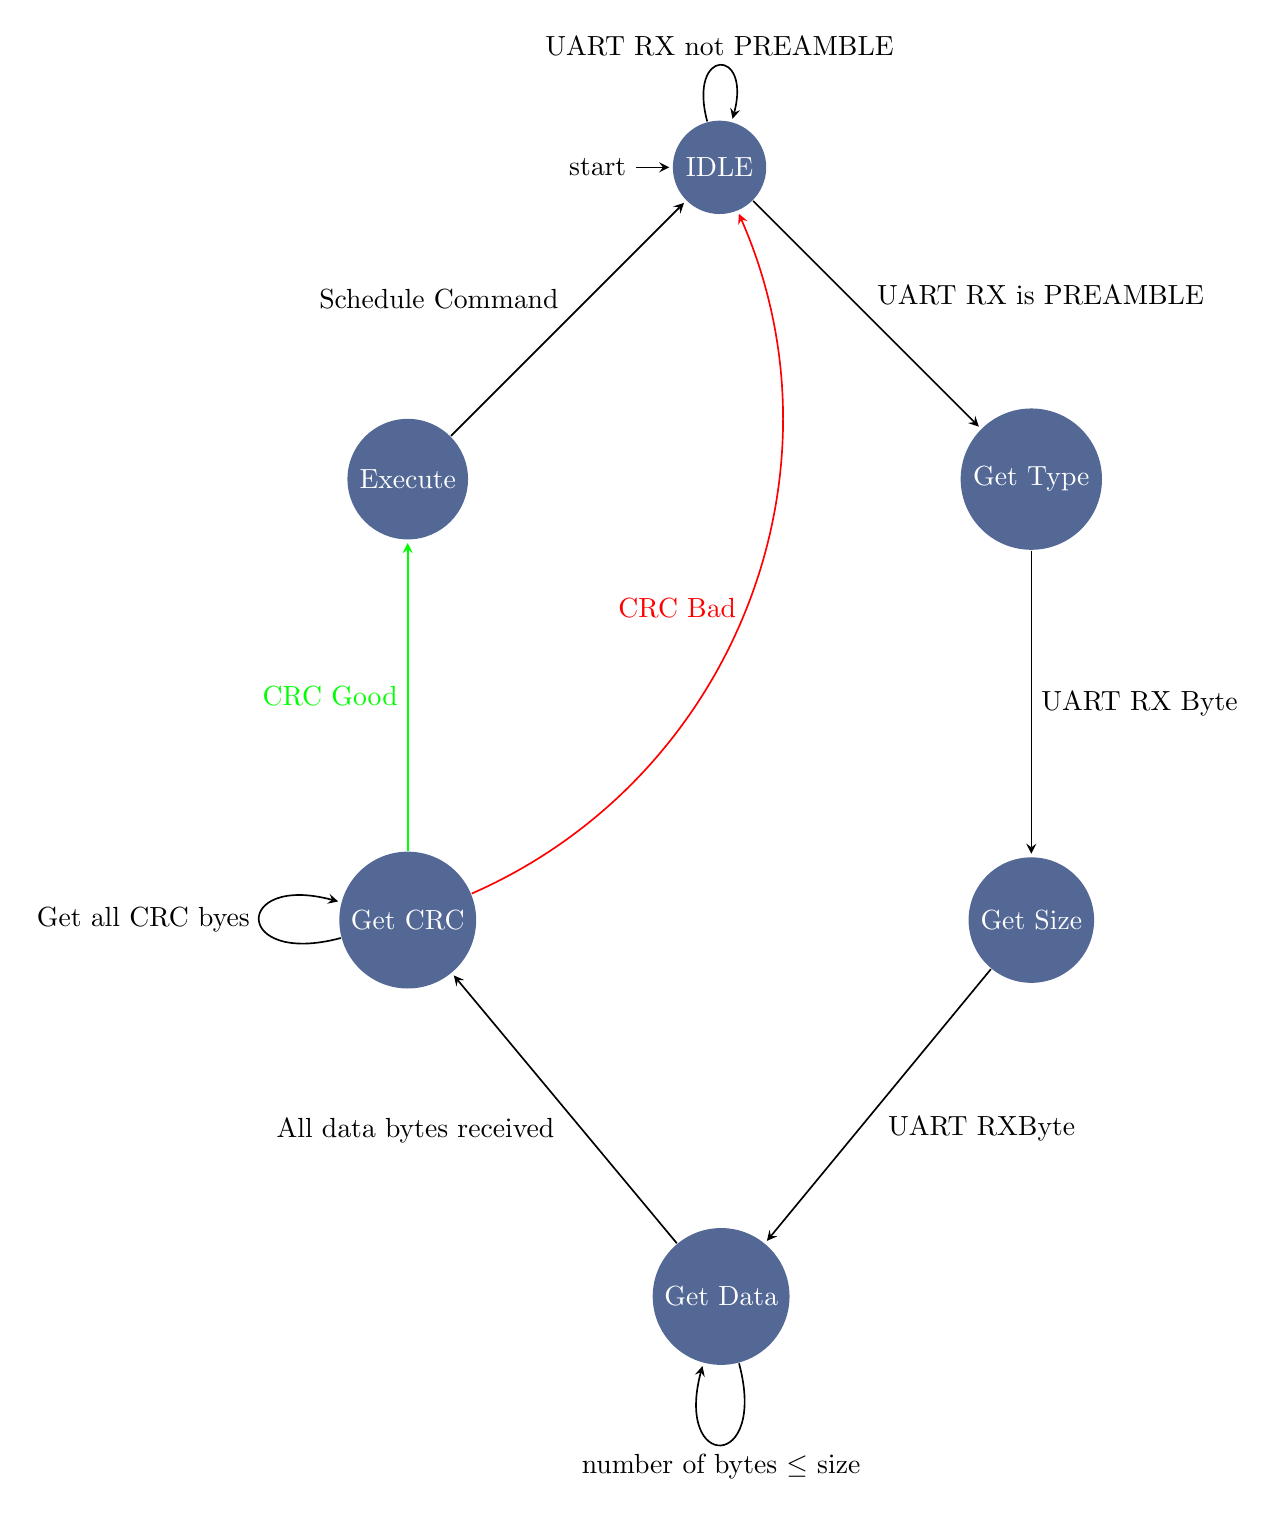
\begin{tikzpicture}[->,>=stealth,shorten >=1pt,auto,node distance=2.8cm,
                    semithick]
  \tikzstyle{every state}=[fill=UCLABlue,draw=none,text=white]

  \node[initial,state] (IDLE)           {IDLE};
  \node[state, minimum size=0, white]         (invisible1)     [below right of=IDLE] {};               
  \node[state]         (GetType)        [below right of=invisible1] {Get Type};
  \node[state, minimum size=0, white]         (invisible3)     [below of=GetType] {};               
  \node[state]         (GetSize)        [below of =invisible3] {Get Size};
  \node[state, minimum size=0, white]         (invisible5)     [below of=GetSize] {};               

  \node[state, minimum size=0, white]         (invisible2)     [below left of=IDLE] {};                 
  \node[state]         (ExecuteCommand) [below left of=invisible2] {Execute};
  \node[state, minimum size=0, white]         (invisible4)     [below of=ExecuteCommand] {};                 
  \node[state]         (GetCRC)         [below of=invisible4]       {Get CRC};
  \node[state, minimum size=0, white]         (invisible6)     [below of=GetCRC] {};                 
  \node[state, xshift=2cm]         (GetData)        [below right of=invisible6] {Get Data};



  \path (IDLE)    edge [loop above] node {UART RX not PREAMBLE} (IDLE)
        (IDLE)    edge           node {UART RX is PREAMBLE} (GetType)
        (GetType) edge           node {UART RX Byte} (GetSize)
        (GetSize) edge           node {UART RX \\Byte} (GetData)
        (GetData) edge [loop below] node {number of bytes $\le$  size} (GetData)
        (GetData) edge           node {All data bytes received} (GetCRC)
        (GetCRC) edge [loop left] node{Get all CRC byes}(GetCRC)
        (GetCRC)  edge [green]         node {CRC Good} (ExecuteCommand)
        (GetCRC)  edge [red, swap, left=10pt, bend right =45]           node {CRC Bad} (IDLE)
        (ExecuteCommand) edge node {Schedule Command}(IDLE)
        ;
\end{tikzpicture}
\newpage

\chapter{Python}
\section{Resources}
\begin{enumerate}
\item Python 3.4
\item PyQT
\item PySerial
\end{enumerate}
\newpage
\section{Environment}
\newpage
\section{Code}
\newpage


\chapter{Working Together}


\end{document}
